\documentclass[11pt]{article}
\usepackage[margin=1in]{geometry}
\usepackage{amsmath,amssymb,amsthm}
\usepackage{booktabs,longtable,array}
\usepackage{graphicx}
\usepackage{float}
\usepackage[hidelinks]{hyperref}
\usepackage{enumitem}

\title{Content-Centric Modeling of Virality, Latent Discussion Pressure, and User Retention on Social Media\\\large An IVFS ODE Model Calibrated on the Higgs Twitter Dataset}
\author{Neel Sarkar \and Piper Scott}
\date{March 2026}

\newtheorem{proposition}{Proposition}
\newtheorem{remark}{Remark}

\begin{document}
\maketitle

\begin{abstract}
We study how platform amplification changes short-run virality and long-run platform health in a content-centric ODE model. The model tracks ignored, viral, fatigued, and suppressed content together with a latent harmful-discussion pressure variable and an active-user pool. The spread block is calibrated on the SNAP Higgs Twitter activity stream using retweet activity, while discussion pressure is linked to same-dataset reply activity and compared against an external toxicity reference scale. The fitted spread model gives a strong empirical match on the main Higgs window and produces a clear threshold in the amplification parameter, with the current estimate at $\alpha_{\mathrm{crit}} \approx 0.3165$. Higher amplification raises long-run viral volume and discussion pressure while lowering long-run user retention. The main limitation is that discussion pressure is proxy-grounded rather than directly observed text toxicity, so the pressure block is only partially identified.
\end{abstract}

\section{Background}
Algorithmic amplification can increase the spread of engaging content while also increasing unhealthy conversation dynamics and long-run user fatigue. That tradeoff motivates the present project. Most simple compartmental social-media models track user states. In contrast, this project treats \emph{content lifecycle states} as the main dynamical objects and then couples them to a latent discussion-pressure state and a user-retention block.

The conceptual goal is to model a rage-bait style platform tradeoff in a way that is both mathematically interpretable and empirically grounded. The spread side of the project is anchored to the SNAP Higgs Twitter activity data, and the pressure side is tied to same-dataset reply behavior rather than literal text-level toxicity labels. This gives a cleaner research path than overclaiming a direct toxicity calibration from Higgs.

\section{Modelling Question}
The main modelling question is:
\begin{quote}
How does platform amplification affect virality, harmful-discussion pressure, and long-run user retention?
\end{quote}
We also ask:
\begin{enumerate}[leftmargin=1.5em]
    \item When does viral spread become self-sustaining?
    \item How sensitive are the long-run outcomes to the pressure block?
    \item Can one same-system dataset support both a spread calibration and a pressure proxy without overclaiming direct toxicity measurement?
\end{enumerate}

\section{Modelling Approach}
We use a six-state IVFS system. The spread block is calibrated first on retweet activity from the Higgs dataset using a reduced helper model. The full IVFS model is then simulated under policy scenarios with different amplification levels. For the pressure block, we do \emph{not} interpret $\tau$ as directly observed toxicity. Instead, we interpret $\tau$ as a latent harmful-discussion or reply-pressure state. Same-dataset reply activity (RE) is used as the main observable proxy, mentions (MT) are used as an auxiliary same-dataset proxy, and the Jigsaw toxicity data is used only as an external reference scale.

This split is deliberate. It makes the report honest now and leaves a stronger research-paper path later, where $\tau$ can be treated as a latent state with multiple noisy observables.

\section{Formulation of the Model}
\subsection{State variables and parameters}
The full model states are:
\begin{center}
\begin{tabular}{>{\raggedright\arraybackslash}p{1.4cm} >{\raggedright\arraybackslash}p{11.2cm}}
\toprule
State & Meaning \\
\midrule
$I$ & ignored or not-yet-viral content \\
$V$ & viral content \\
$F$ & fatigued content \\
$S$ & suppressed / moderated content \\
$\tau$ & latent harmful-discussion pressure \\
$U$ & active users \\
\bottomrule
\end{tabular}
\end{center}

The fixed scenario parameters currently used in code are shown in Table~\ref{tab:params}.

\begin{table}[H]
\centering
\caption{Core IVFS parameters used in the current implementation.}
\label{tab:params}
\begin{tabular}{cccc}
\toprule
Parameter & Value & Interpretation & Role \\
\midrule
$\kappa$ & $0.8$ & pressure effect on amplification & fixed scenario parameter \\
$\eta$ & $0.3$ & pressure effect on fatigue & fixed scenario parameter \\
$\phi$ & $0.056$ & viral-to-pressure forcing & baseline scenario parameter \\
$\psi$ & $0.1$ & pressure relaxation rate & baseline scenario parameter \\
$\rho$ & $0.06$ & content injection scale & fixed scenario parameter \\
$\lambda_u$ & $0.02$ & user attrition scale & fixed scenario parameter \\
$\nu$ & $1.0$ & user replenishment & fixed scenario parameter \\
$\mu_c$ & $0.01$ & natural content decay & fixed scenario parameter \\
$\delta$ & $0.05$ & moderation / suppression rate & fixed scenario parameter \\
$w$ & $10.0$ & pressure effect on user loss & fixed scenario parameter \\
\bottomrule
\end{tabular}
\end{table}

\subsection{IVFS equations}
The model implemented in the current code is
\begin{align*}
\dot I &= \frac{\rho U}{1+U} - \beta_{\mathrm{eff}} I V - (\delta + \mu_c) I, \\
\dot V &= \beta_{\mathrm{eff}} I V - \gamma_{\mathrm{eff}} V - \mu_c V, \\
\dot F &= \gamma_{\mathrm{eff}} V - \mu_c F, \\
\dot S &= \delta I - \mu_c S, \\
\dot \tau &= \phi V - \psi \tau, \\
\dot U &= \nu - \lambda_u (1+w\tau) U,
\end{align*}
with
\[
\beta_{\mathrm{eff}} = \alpha \beta_0 (1+\kappa \tau), \qquad
\gamma_{\mathrm{eff}} = \gamma_0 (1+\eta \tau).
\]
The saturating inflow $\rho U/(1+U)$ is important. A purely linear inflow term made the content input unrealistically large in the implemented simulations, so the saturating form is used throughout the current project code.

Although the full state vector is six-dimensional, the active feedback loop is mainly driven by $(I,V,\tau,U)$. The $F$ and $S$ compartments are sinks that help interpret the lifecycle, but they do not feed back into the main spread-pressure-user block.

\subsection{Threshold quantity and equilibria}
At the disease-free equilibrium (DFE), we have
\[
U_{\mathrm{DFE}} = \frac{\nu}{\lambda_u}, \qquad
I_{\mathrm{DFE}} = \frac{\rho U_{\mathrm{DFE}}}{(1+U_{\mathrm{DFE}})(\delta+\mu_c)}.
\]
Linearizing the viral equation around the DFE gives the threshold quantity
\[
\mathcal R_0 = \frac{\alpha \beta_0 I_{\mathrm{DFE}}}{\gamma_0+\mu_c}.
\]
With the current Higgs-based calibration, the threshold occurs at
\[
\alpha_{\mathrm{crit}} \approx 0.3165.
\]
So the health-first scenario ($\alpha=0.2$) is subcritical, while the moderate and engagement-first scenarios remain supercritical.

\section{Data and Calibration}
\subsection{Higgs activity data}
The main dataset is the SNAP Higgs Twitter activity stream. The activity file records tuples of the form
\[
\texttt{userA userB timestamp interaction},
\]
where the interaction is one of \texttt{RT}, \texttt{RE}, or \texttt{MT}. There is no tweet text in the file. For the current dataset version used in the repository, the activity counts are:
\begin{itemize}[leftmargin=1.5em]
    \item total rows: $563{,}069$
    \item retweets (RT): $354{,}930$
    \item replies (RE): $36{,}902$
    \item mentions (MT): $171{,}237$
\end{itemize}
The main retweet spike peaks at hour $78$ with $30{,}602$ retweets. The calibration window used in the code is the 100-hour window from hour 68 to hour 167, centered around the main spike.

\subsection{Reduced calibration model}
The spread calibration is carried out with a reduced IVF helper model. A decaying exogenous seed term is added to improve the fit of the late tail:
\[
\lambda(t) = \lambda_0 e^{-d_\lambda t}.
\]
The fitted helper parameters are $(\beta_0,\gamma_0,\lambda_0,d_\lambda,V_0)$, while the policy parameters in the full IVFS system are held fixed in the scenario stage.

The current fitted spread values are:
\[
\beta_0 = 1.000073,\qquad \gamma_0 = 0.300283,\qquad
\lambda_0 = 0.199996,\qquad d_\lambda = 0.044641.
\]

\subsection{Observed proxy for discussion pressure}
The most important modelling decision in this draft is the interpretation of $\tau$. We define $\tau(t)$ as a latent harmful-discussion pressure state rather than directly observed text toxicity. Higgs replies (RE) give the main same-dataset proxy for that pressure. Mentions (MT) are used as an auxiliary same-dataset signal, and the normalized reply-rate proxy $RE/(RT+1)$ is used to separate reply intensity from raw spread volume.

The code now constructs a small proxy family and chooses the best same-dataset fit among:
\begin{itemize}[leftmargin=1.5em]
    \item a smoothed RE proxy,
    \item a smoothed reply-rate proxy $RE/(RT+1)$,
    \item a composite proxy $0.55\,RE + 0.30\,RE/(RT+1) + 0.15\,MT$ after normalization.
\end{itemize}
In the present run, the RE proxy is the best-supported same-dataset target for the latent-pressure fit. Under the current one-timescale pressure block, the unconstrained proxy-fit quality is $R^2 \approx 0.7422$ for the RE proxy, compared with $R^2 \approx -0.5302$ for the composite proxy and $R^2 \approx -1.1419$ for the reply-rate proxy. That ranking is why the report highlights RE rather than claiming that any smoothed interaction measure is equally defensible.

\subsection{External toxicity reference}
The file [data/toxicity/train.csv] in the repository is a Jigsaw-style toxicity dataset. It is not used as a spread dataset and it is not treated as a same-system calibration source. Instead, it gives an external reference scale for the size of $\tau$. The mean toxicity rate in that file is approximately $0.101679$, which implies an external-scale comparison value of $\phi \approx 0.1459$ if $\psi$ is fixed at $0.1$ and the moderate-scenario equilibrium viral volume is used for scaling.

\subsection{Calibration diagnostics}
The main spread diagnostics from the current implementation are:
\begin{itemize}[leftmargin=1.5em]
    \item weighted loss: $0.002286$
    \item full-window $R^2$: $0.9247$
    \item spike-window $R^2$: $0.8891$
    \item tail mean bias: $+0.0043$
\end{itemize}
Because the calibration window itself is the full 100-hour fitting window, the fit-window and full-window $R^2$ values coincide in the current run.
The spread benchmark against SIR also favors the current IVF helper model on the Higgs window. The repository additionally contains parametric bootstrap intervals and local profile-likelihood curves, both of which support practical identifiability of the spread parameters.

Figure~\ref{fig:cal} shows the calibration diagnostics. Figure~\ref{fig:taucompare} shows the same-dataset pressure-proxy comparison. Figure~\ref{fig:results} shows the main policy results.

\begin{figure}[H]
\centering
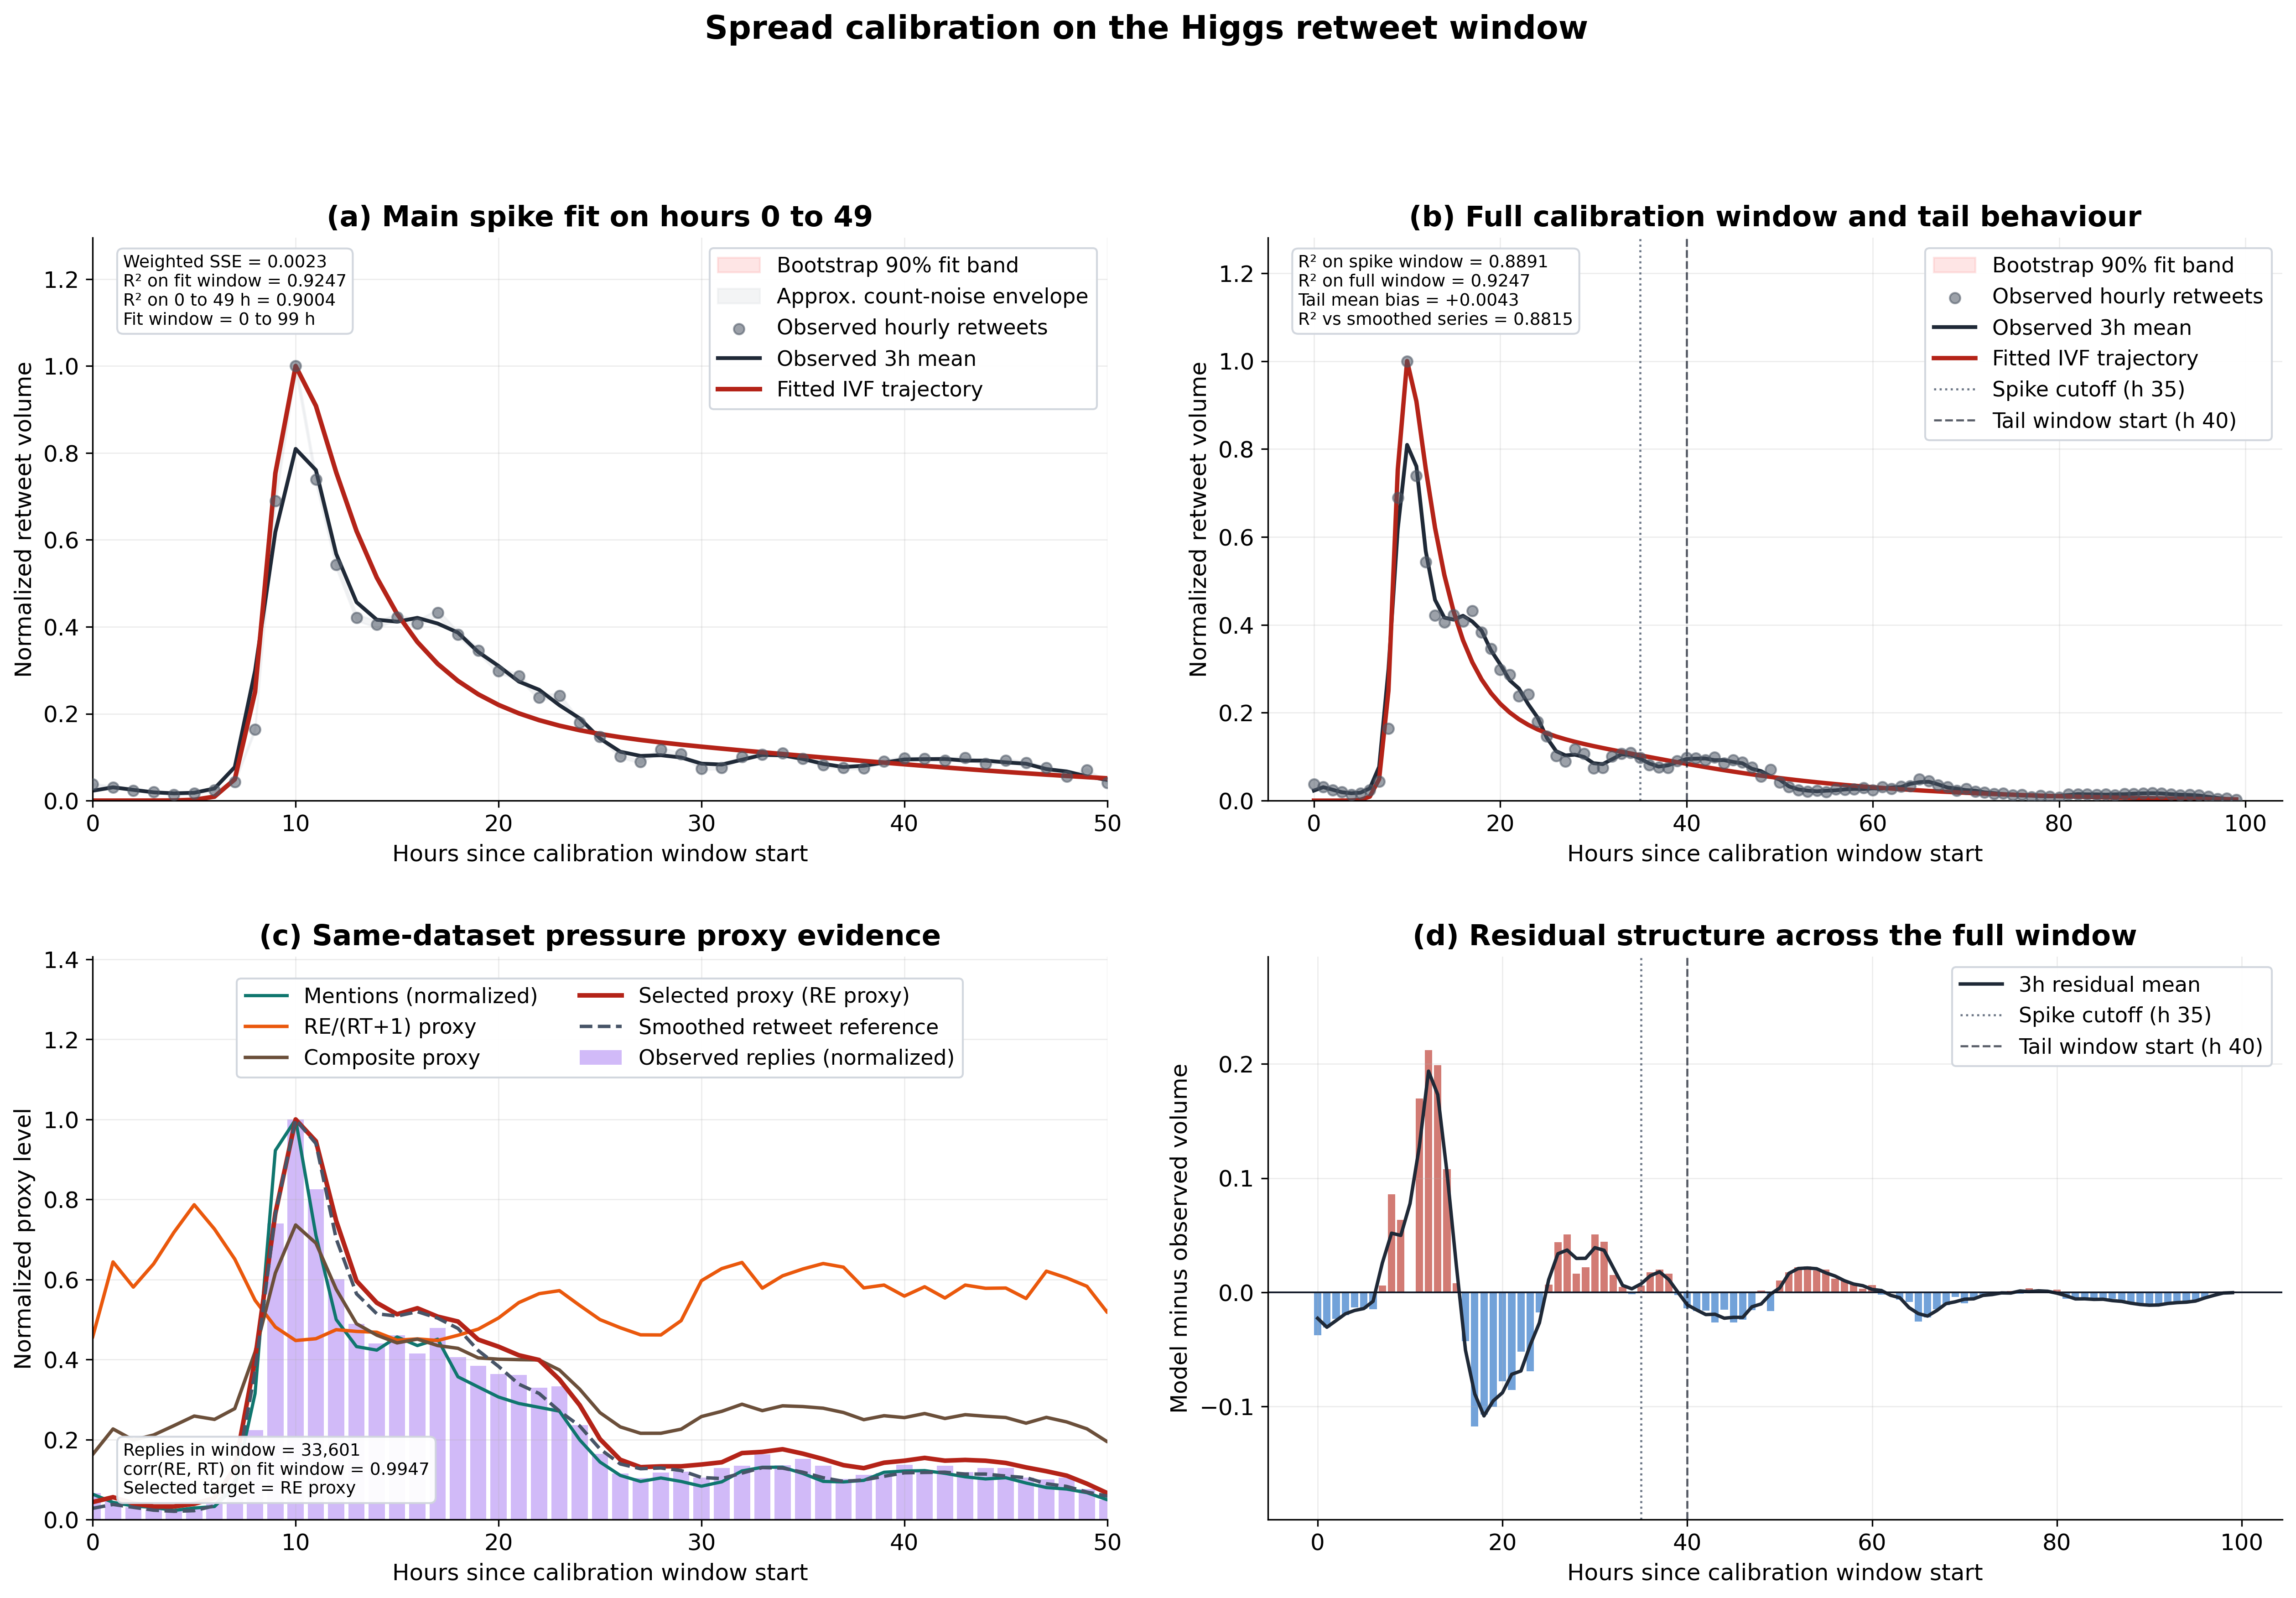
\includegraphics[width=0.95\textwidth]{assets/apm348_calibration_diagnostics.png}
\caption{Calibration diagnostics for the Higgs fit, including the retweet calibration window, tail behavior, and the same-dataset latent-pressure proxy family.}
\label{fig:cal}
\end{figure}

\begin{figure}[H]
\centering
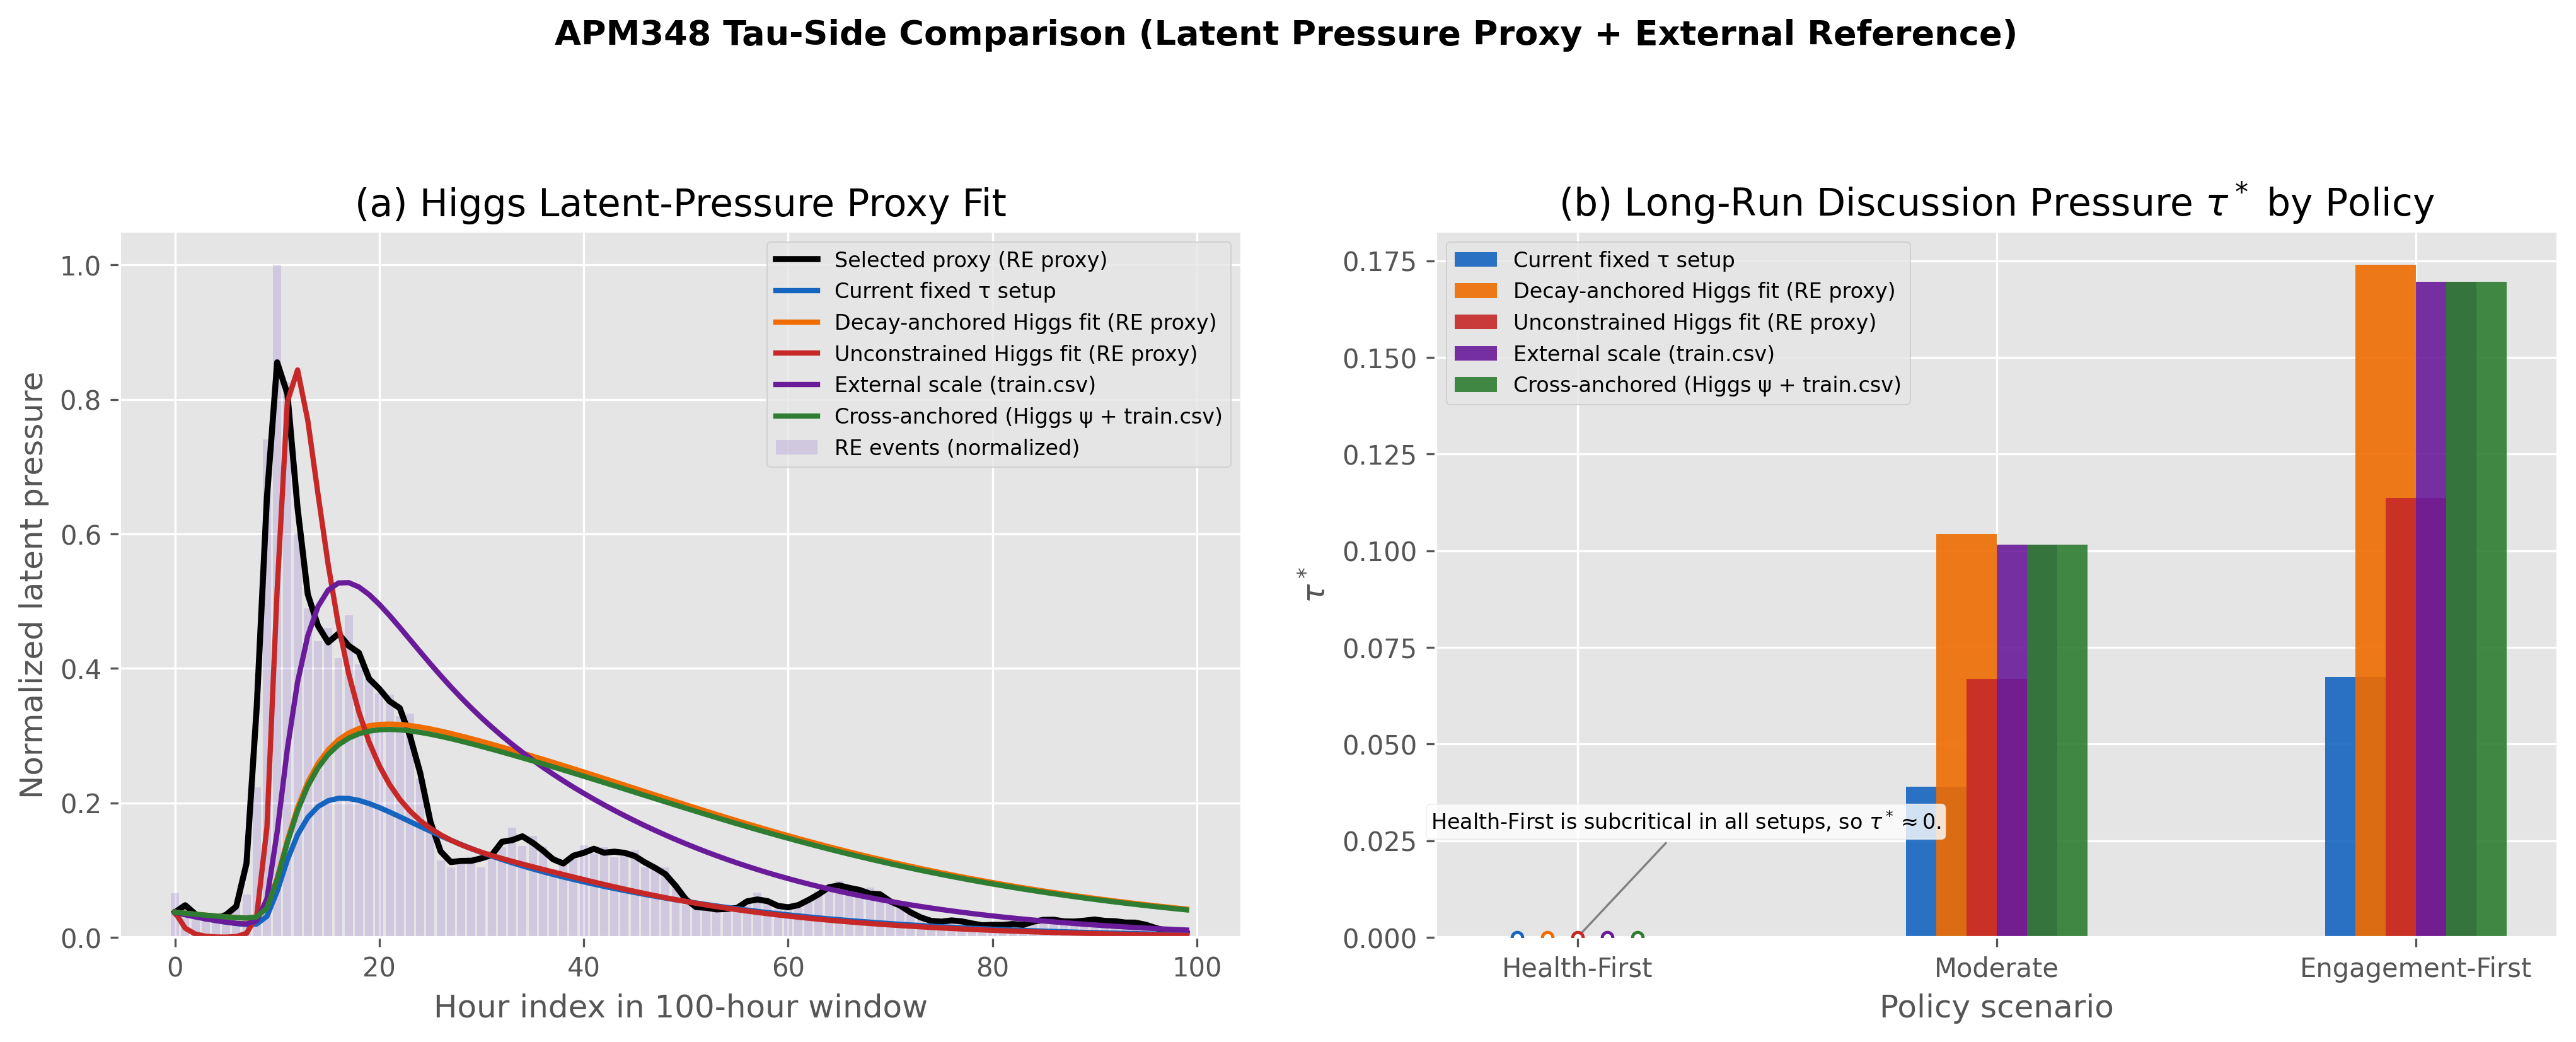
\includegraphics[width=0.9\textwidth]{assets/tau_proxy_comparison.png}
\caption{Latent-pressure proxy comparison. In the current run the black reference curve is the selected RE proxy, and the same spread fit is compared against the baseline pressure block, a decay-anchored same-dataset RE fit, an unconstrained same-dataset RE fit, an external reference scale, and the cross-anchored configuration (Higgs $\psi$ combined with external gain ratio $r=\phi/\psi$). The cross-anchored case is the preferred jointly-grounded anchor. The Health-First case is subcritical in all setups, so its long-run pressure remains essentially zero.}
\label{fig:taucompare}
\end{figure}

\section{Analysis of the Model}
\subsection{Nonnegativity}
\begin{proposition}
If the initial state satisfies
\[
I(0),V(0),F(0),S(0),\tau(0),U(0) \ge 0,
\]
then the solution remains componentwise nonnegative for as long as it exists.
\end{proposition}

\begin{proof}[Proof sketch]
Each coordinate hyperplane is inward-pointing or tangent. At $I=0$, we have $\dot I = \rho U/(1+U) \ge 0$. At $V=0$, we have $\dot V = 0$. At $F=0$, $\dot F = \gamma_{\mathrm{eff}}V \ge 0$. At $S=0$, $\dot S = \delta I \ge 0$. At $\tau=0$, $\dot\tau = \phi V \ge 0$. At $U=0$, $\dot U = \nu > 0$. Therefore the nonnegative orthant is positively invariant.
\end{proof}

\subsection{Boundedness and invariant region}
\begin{proposition}
Solutions of the IVFS system with nonnegative initial data enter a bounded positively invariant region.
\end{proposition}

\begin{proof}[Proof sketch]
First, 
\[
\dot U = \nu - \lambda_u(1+w\tau)U \le \nu - \lambda_u U,
\]
so $U(t)$ is bounded above by $\max\{U(0),\nu/\lambda_u\}$. Next define the total content mass
\[
C = I+V+F+S.
\]
Then the internal transfer terms cancel and
\[
\dot C = \frac{\rho U}{1+U} - \mu_c C \le \rho U_{\max} - \mu_c C,
\]
so $C$ is bounded. Since $V \le C$, the pressure equation gives
\[
\dot\tau \le \phi C_{\max} - \psi \tau,
\]
so $\tau$ is bounded as well. Hence all state variables remain in a compact feasible region after a transient.
\end{proof}

\subsection{Disease-free threshold and positive equilibrium}
\begin{proposition}
The DFE loses stability when $\mathcal R_0$ crosses $1$, where
\[
\mathcal R_0 = \frac{\alpha \beta_0 I_{\mathrm{DFE}}}{\gamma_0+\mu_c}.
\]
Under the current calibration this gives $\alpha_{\mathrm{crit}} \approx 0.3165$.
\end{proposition}

\begin{proof}[Proof sketch]
At the DFE we have $\tau=0$ and $V=0$, so the linearized viral equation is
\[
\dot V \approx (\alpha\beta_0 I_{\mathrm{DFE}} - \gamma_0 - \mu_c)V.
\]
The sign of the coefficient determines local invasion or decay, giving the threshold expression above.
\end{proof}

\subsection{Local stability}
The repository numerically evaluates the Jacobian of the full six-state system. The present numerical results show:
\begin{itemize}[leftmargin=1.5em]
    \item at $\alpha=0.2$, $\mathcal R_0 \approx 0.632$ and no positive equilibrium is found;
    \item at $\alpha=0.5$, $\mathcal R_0 \approx 1.580$ and the positive equilibrium is locally stable;
    \item at $\alpha=0.9$, $\mathcal R_0 \approx 2.844$ and the positive equilibrium is locally stable.
\end{itemize}
In the current numerical Jacobian output, the leading real part at the positive equilibrium is $-0.01$, which corresponds to the decoupled sink eigenvalue from the content-decay block. A fully symbolic local-stability theorem is still future work, but the numerical local checks are already consistent with the threshold picture.

\begin{remark}
A stronger research-paper version of this section should replace the current threshold sketch with a full next-generation-matrix derivation and should turn the Jacobian discussion into explicit theorem statements.
\end{remark}

\section{Numerical Results}
\subsection{Policy scenarios}
The project compares three policy settings:
\begin{itemize}[leftmargin=1.5em]
    \item engagement-first: $\alpha=0.9$
    \item moderate: $\alpha=0.5$
    \item health-first: $\alpha=0.2$
\end{itemize}
The long-run scenario outputs under the baseline pressure block are shown in Table~\ref{tab:scenarios}.

\begin{table}[H]
\centering
\caption{Long-run scenario outputs from the current baseline pressure setup.}
\label{tab:scenarios}
\begin{tabular}{lcccc}
\toprule
Scenario & $\mathcal R_0$ & $V^*$ & $\tau^*$ & $U^*$ \\
\midrule
Engagement-first ($\alpha=0.9$) & $2.84$ & $0.120267$ & $0.067350$ & $29.8776$ \\
Moderate ($\alpha=0.5$) & $1.58$ & $0.069674$ & $0.039018$ & $35.9667$ \\
Health-first ($\alpha=0.2$) & $0.63$ & $0.000000$ & $0.000000$ & $50.0000$ \\
\bottomrule
\end{tabular}
\end{table}

The health-first scenario is now subcritical and therefore suppresses sustained virality. The moderate and engagement-first scenarios both remain supercritical, but the engagement-first case has higher long-run viral volume and higher pressure together with lower user retention.

\subsection{Continuation in amplification}
The continuation sweep over $\alpha \in [0.05,1.0]$ shows a clear threshold crossing near $\alpha\approx 0.3165$. Below that point, the long-run viral and pressure states collapse to zero. Above it, both $\tau^*$ and $V^*$ increase with amplification, while $U^*$ decreases. The long-run engagement measure
\[
E^* = \alpha V^* U^*
\]
peaks at the upper end of the tested $\alpha$ range in the present parameter regime.

\subsection{Pressure robustness}
The code now performs two relevant robustness checks:
\begin{enumerate}[leftmargin=1.5em]
    \item a $\phi$ sweep with $\psi$ fixed,
    \item a same-dataset proxy comparison across several latent-pressure targets.
\end{enumerate}
Across the $\phi$ sweep, the qualitative ordering of the three policy scenarios is preserved: engagement-first always yields the highest long-run pressure, moderate stays in the middle, and health-first stays lowest. That means the main policy ranking is not an artifact of one single baseline choice for $\phi$.

This $\phi$ sweep is a \emph{local} robustness check around the baseline scenario block with $\psi$ held fixed at $0.1$, so it is designed to compare the current baseline $\phi=0.056$ against the external-reference scale $\phi\approx 0.1459$. It is not intended to uniquely identify the same-dataset RE-based fit, because that fit changes both $\phi$ and $\psi$ simultaneously and the Higgs reply proxy does not separately pin down the forcing and decay timescales.

For the same-dataset proxy family, the present implementation selects the RE proxy as the most interpretable and best-supported same-dataset target. The report now shows \emph{two} same-dataset RE-based fits rather than pretending there is a unique calibrated pair. The decay-anchored fit uses the empirical reply-decay timescale and gives approximately
\[
\phi \approx 0.0613, \qquad \psi \approx 0.0409,
\]
with anchored proxy-fit quality $R^2 \approx 0.0952$. The unconstrained same-dataset fit gives
\[
\phi \approx 0.9596, \qquad \psi \approx 1.0000,
\]
with proxy-fit quality $R^2 \approx 0.7422$. The wide gap between these two same-dataset fits is itself the key identifiability result: the spread data and the reply proxy support the qualitative pressure story, but they do not uniquely determine one definitive $(\phi,\psi)$ pair under the present one-timescale pressure block.

\textbf{Cross-anchored resolution.}
This identification problem has a principled solution when an external toxicity reference is available.
The key observation is that the normalized proxy shape identifies $\psi$ (the pressure decay
timescale) via the post-peak decay slope of the RE activity, while the external toxicity rate
anchors the steady-state gain ratio $r = \phi/\psi$ via $r = \tau_{\mathrm{ref}}/V^*_{\mathrm{mod}}$.
Combining these two independent pieces of information gives the \emph{cross-anchored} configuration:
\[
\psi_{\mathrm{cross}} \approx 0.0409 \quad \text{(Higgs RE decay timescale)},
\qquad
r = \frac{\phi_{\mathrm{ext}}}{\psi_{\mathrm{default}}} \approx 1.46 \quad \text{(external reference)},
\]
\[
\phi_{\mathrm{cross}} = r \cdot \psi_{\mathrm{cross}} \approx 1.46 \times 0.0409 \approx 0.0597.
\]
By construction, the cross-anchored equilibrium satisfies $\tau^* = r \cdot V^*_{\mathrm{mod}} \approx \tau_{\mathrm{ref}}$
at the moderate scenario, matching the external toxicity reference, while its transient pressure dynamics
follow the empirically estimated Higgs relaxation timescale rather than the arbitrary default $\psi=0.1$.
The cross-anchored configuration is now included in the tau comparison figure as the preferred
jointly-grounded anchor.

\begin{figure}[H]
\centering
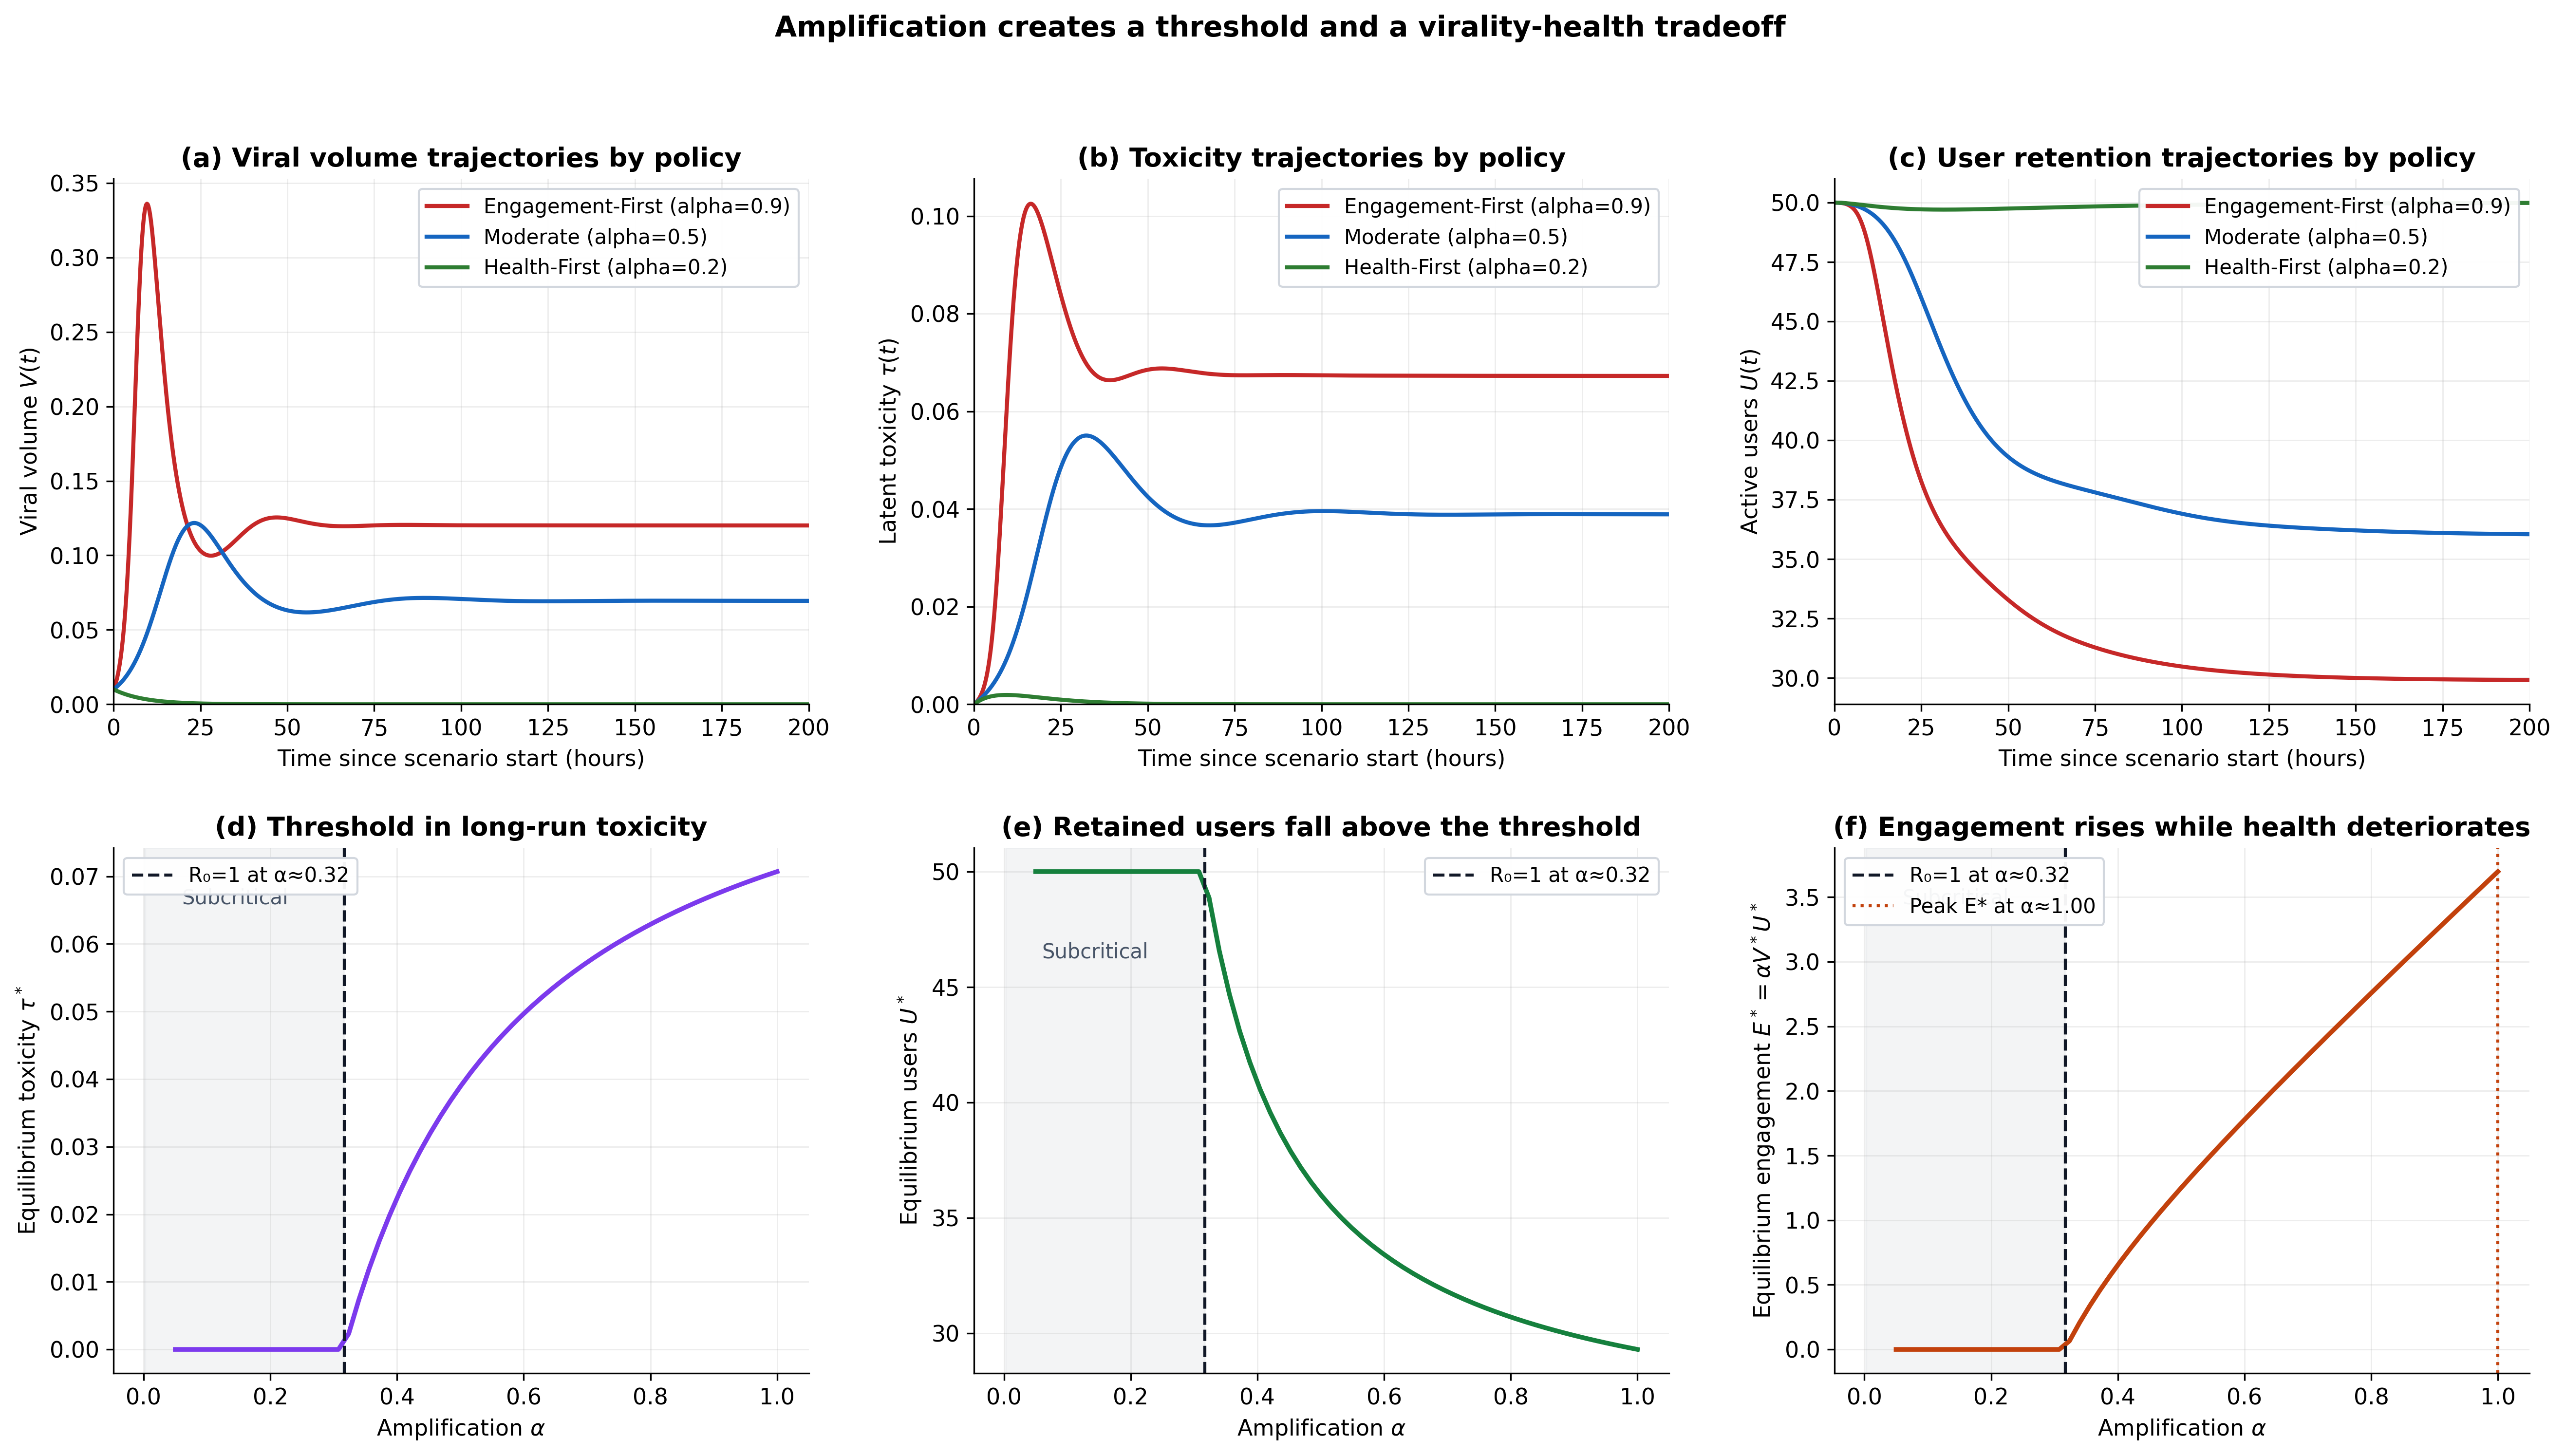
\includegraphics[width=0.95\textwidth]{assets/apm348_results.png}
\caption{Policy scenarios and continuation results for the current IVFS implementation.}
\label{fig:results}
\end{figure}

\section{Limitations}
The current report has several important limitations.
\begin{enumerate}[leftmargin=1.5em]
    \item The spread calibration is based on one main Higgs event window.
    \item Higgs does not contain text, so the pressure block is proxy-grounded rather than directly text-calibrated.
    \item The latent-pressure parameters $\phi$ and $\psi$ are only partially identified from the same-dataset proxy alone. The cross-anchored configuration addresses this by combining the Higgs decay timescale with the external toxicity reference, but a formally identified latent observation model would require a richer multi-timescale data structure.
    \item The model assumes homogeneous mixing and deterministic dynamics.
    \item The threshold quantity used here comes from DFE linearization; a more formal next-generation-matrix derivation is still desirable for a journal version.
\end{enumerate}
These limitations do not invalidate the present report, but they do set the agenda for the next research stage.

\section{Conclusion}
This report develops a content-centric IVFS model for virality, latent discussion pressure, and user retention on social media. The spread side is strongly grounded by the Higgs retweet data, and the fitted helper model produces a clear threshold in the amplification parameter. The policy simulations show the expected tradeoff: stronger amplification raises long-run viral volume and discussion pressure while lowering user retention. The most important conceptual improvement in the present draft is the treatment of $\tau$ as a latent harmful-discussion pressure state rather than as directly observed toxicity. That framing makes the current empirical package honest and usable now, while still leaving a clear path toward a stronger research paper.

\appendix
\section{Reproducibility notes}
The main scripts in the repository are:
\begin{verbatim}
python code/ivfs_validation.py
python code/equilibrium_analysis.py
python code/benchmark_models.py
python code/toxicity_calibration.py
\end{verbatim}
The main outputs used in this report are written to the \texttt{assets/} directory.

\section{Immediate research-paper upgrades}
The clearest next upgrades are:
\begin{enumerate}[leftmargin=1.5em]
    \item a full next-generation-matrix derivation of $\mathcal R_0$;
    \item theorem-level local and global stability results;
    \item a latent observation model for $\tau$ with RE and MT as noisy observables;
    \item multi-cascade spread validation beyond the main Higgs spike.
\end{enumerate}

\begingroup
\footnotesize
\begin{thebibliography}{9}
\bibitem{snap}
Stanford Network Analysis Project.
Higgs Twitter Dataset.
\url{https://snap.stanford.edu/data/higgs-twitter.html}.

\bibitem{domenico2013}
M.~De Domenico, A.~Lima, P.~Mougel, and M.~Musolesi.
The anatomy of a scientific rumor.
\textit{Scientific Reports}, 3:2980, 2013.

\bibitem{brady2017}
W.~J.~Brady, J.~A.~Wills, J.~T.~Jost, J.~A.~Tucker, and J.~J.~Van~Bavel.
Emotion shapes the diffusion of moralized content in social networks.
\textit{PNAS}, 114(28):7313--7318, 2017.

\bibitem{huszar2022}
F.~Husz\'ar et al.
Algorithmic amplification of politics on Twitter.
\textit{PNAS}, 119(1):e2025334119, 2022.

\bibitem{milli2025}
S.~Milli et al.
Engagement, user satisfaction, and the amplification of divisive content on social media.
PNAS Nexus, 4(3):pgaf062, 2025.

\bibitem{maleki2022}
M.~Maleki, V.~Mead, and N.~Agarwal.
Applying an epidemiological model to evaluate the propagation of toxicity on Twitter.
In \textit{HICSS-55}, 2022.

\bibitem{addai2025}
E.~Addai, N.~Agarwal, and N.~Yousefi.
Modeling and simulation of interventions' effect on the spread of toxicity in social media.
\textit{Online Social Networks and Media}, 46:100309, 2025.

\bibitem{borkan2019}
D.~Borkan, L.~Dixon, J.~Sorensen, N.~Thain, and L.~Vasserman.
Nuanced metrics for measuring unintended bias with real data for text classification.
In \textit{WWW Companion}, 2019.
\end{thebibliography}
\endgroup

\end{document}
